
Attention now turns to the \emph{detection} of replay spoofing attacks.  Given that only little work has investigated ASV vulnerabilities to such attacks, it is hardly surprising that work to develop anti-spoofing countermeasures is similarly limited.  This section briefly reviews that past work and then describes two particular replay countermeasures which are explored further in this paper through comparative experiments.

One obvious approach to replay detection involves challenge-response systems which require the speaker to utter a prompted phrase~\cite{Petrovska1998}. 
Challenge-response mechanisms are a form of passive countermeasure.
While having potential in preventing some forms of replay attack for some ASV systems, challenge-response countermeasures are not without negative impacts on usability which may render them undesirable for other ASV systems.

Active countermeasures have also been proposed.
One such approach involves the storing of previous access attempts and their comparison to new attempts~\cite{Shang2010}.
New access attempts which are deemed too close to previous attempts are rejected.
A somewhat similar technique is proposed in~\cite{Wu2014}, where the authors compare spectral bitmaps between access trials and previously stored recordings in a text-dependent ASV scenario.
%The detection of high similarity was shown to serve as an effective means of identifying replay attack. 
% albeit in a rather constrained scenario.   <-- replace after review

Other, more generally applicable methods not restricted to any particular ASV scenario are based on the detection of unexpected channel artefacts indicative of recording and replaying.
Two such algorithms were reported in~\cite{Wang2011} for which the EER for a baseline GMM-UBM system was shown to decrease from 40\% to 10\% with active countermeasures.  Channel detection is the basis of the first approach investigated further in this paper.



\subsection{Far-field channel detection}

Many scenarios in which user authentication is performed by ASV involve so-called close-talk speech, i.e.\ situations where speech is collected from an in-situ or closely positioned microphone.  Examples include telephone and logical access scenarios or critical infrastructure protection and physical access scenarios.  In contrast, since they are likely to be collected surreptitiously or at-distance, replay recordings will exhibit far-field channel effects, effects which can be measured and consequently used to detect replayed speech.  

This idea was first investigated in~\cite{Villalba2011}.  The work compared close-talk and far-field speech signals parametrised according to 12 channel-sensitive features:


\begin{itemize}
\item spectral ratio -- sub-band energy ratio from 0-2~kHz and from 2-4~kHz; 
\item low frequency ratio -- sub-band energy ratio from 100-300~Hz and from 300-500~Hz, calculated using speech frames only;
\item total modulation index, and
\item nine sub-band modulation indices -- see~\cite{Villalba2011} for precise sub-band bandwidths.
\end{itemize}


The spectral ratio reflect reflects the level of spectrum flattening or noise and reverberation introduced by far-field recording.  The low frequency ratio reflects the level of high-pass filtering, an artefact typical of speech signals  produced by small loudspeakers.  The total and sub-band modulation indices reflect the level of additive and, specifically, coloured noise; higher levels of noise present in replay recordings result in lower than average modulation indices.  Experiments showed that far-field recordings could be detected with 90\%  accuracy.  {\bfseries what classifier?}



\subsection{Local binary patterns}


\begin{figure*}
	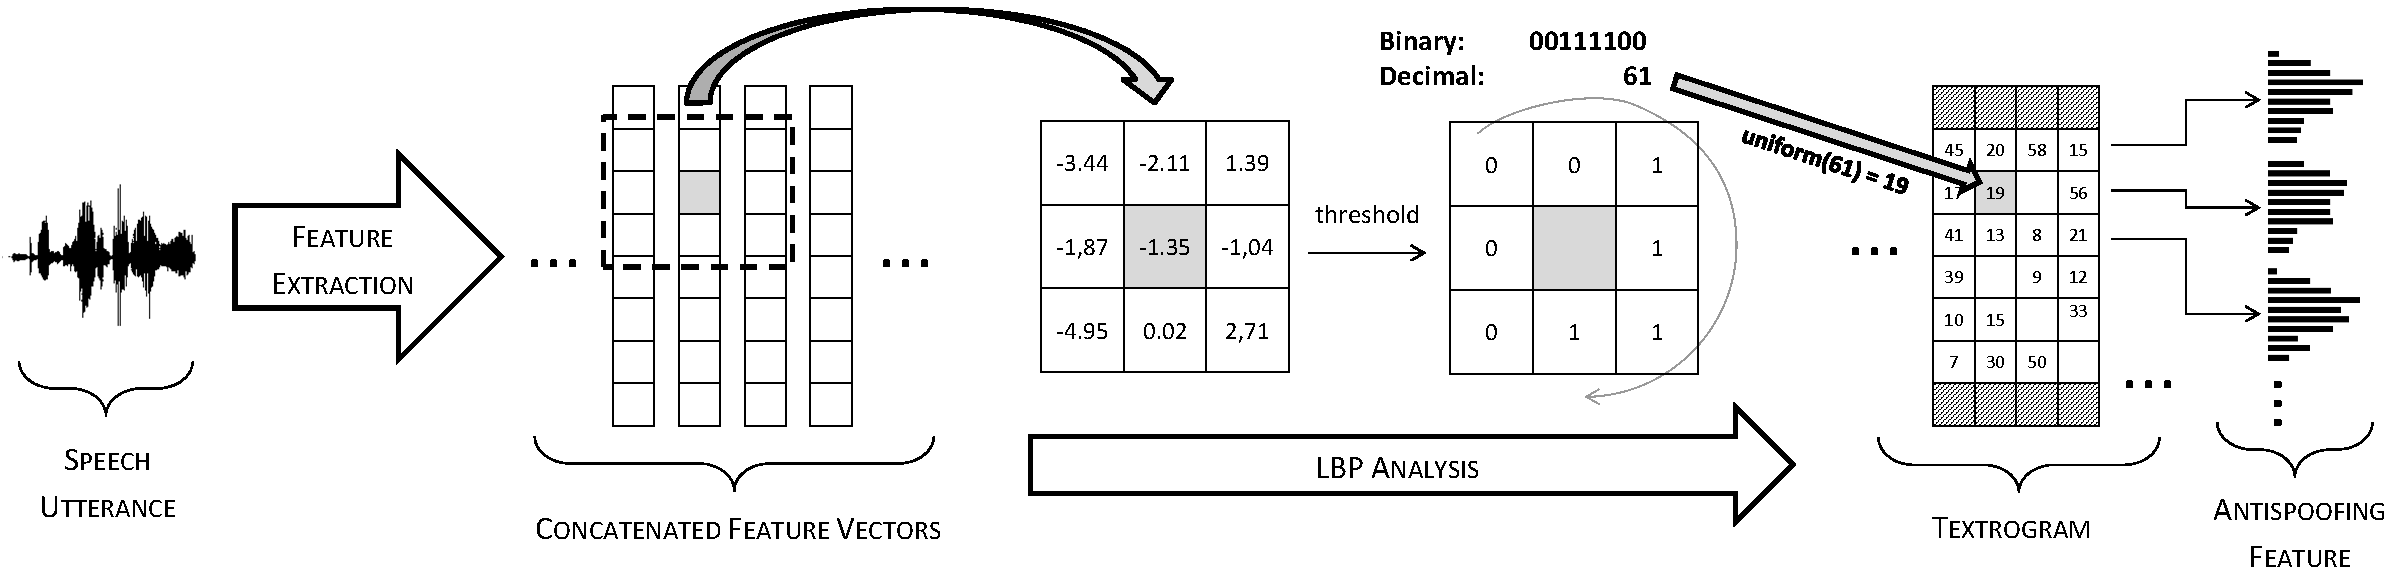
\includegraphics[width=1\linewidth]{Figs/LBPfeature.pdf}
	\caption{Schematic diagram of LBP-based feature extraction.}
	\label{fig:LBPfeature}
\end{figure*}


Another method, proposed in~\cite{Alegre2013a}, uses local binary patterns (LBP) technique. It is based on the hypothesis that modifications made through spoofing disturb the natural 'texture' of genuine speech. This technique was adopted from a standard texture analysis approach, known in image processing~\cite{Ojala2002}, to a 2-dimensional 'image' of a speech utterance, where the image is a mel-scaled cepstrogram appended with dynamic features. 

The standard LBP operator is a non-parametric 3x3 kernel which assigns a binary code to each pixel in an image according to the comparison of its intensity value to that of its eight surrounding pixels~\cite{Ojala2002}. This procedure is illustrated in Fig.~\ref{fig:LBPfeature}.  A binary value of '1' is assigned when the intensity of neighbouring pixels (here feature components) is higher, whereas a value of '0' is assigned when neighbouring pixels are of lower or equal intensity. Each pixel is thus assigned one of $2^8=256$ binary patterns.

LBPs are determined for each pixel in the mel-scaled cepstrogram thus resulting in a new matrix of reduced dynamic range, here referred to as a 'textrogram'.  The textrogram captures short-time feature motion beyond that in conventional dynamic parametrisation.  The LBP-based countermeasure is based on concatenated histograms formed from the pixel values across each row in the textrogram.  The histograms are individually normalised and their resulting bin values are stacked vertically to obtain a new vector in the same manner as GMM mean-vectors are stacked to form supervectors.  

This method turned out to be  highly effective for artificial signals, yielding 0\% EER for the five tested ASVs, very effective for speech synthesis attacks (EER values below 1\%) and quite effective for voice conversion -- EERs less than 7\%. Considering the fact that the LBP-based countermeasure hardly relies on prior knowledge on the attack, in this work we decided to try to use it also as a countermeasure against replay attacks.



